\let\textcircled=\pgftextcircled
\chapter{Introduction}\label{ch:intro}%    test ~\parencite{pozyx2018pozyx}
%    \lipsum[2-4]
    \initial{I}n recent years Unmanned aerial vehicle(UAV) usages has grown exponentially becoming common in industry and households~\cite{custers2016drones}.
    A major part of UAV applications is their ability to localise themselves in the given environment with acceptable precision and accuracy.
    This is a common requirement in any robotic system but UAV's are often limited by strict payload requirements and therefore have to rely on sensors that are lightweight and robust.
    ~\citep{ardupilotadvanced} gives a good summary of physical components that are used in various vehicles but a UAV system, specifically, a quadrotor system cab be summarised as follows:
    \begin{itemize}
        \item Rotor build - This section contains parts that should be researched based on the size and physical requirements of the drone.
        These include: brushless motors, electronic speed controllers, frame size.
        \item Flight controller unit(FCU) - This acts as the mother board and brain of the quadrotor system.
        It collates data from various sensors, sends commands to the motors and if there is a companion computer is attached collects and sends data to it.
        Commercial FCU's contain the various control systems and laws required for stable flight and movement.
        Most have an array of sensors built in.
        \item Sensors - These vary from from inertial, positioning, barometric and camera.
        Aside from inertial and barometric sensors that are present in most FCU's, sensors are chosen based on the environment and use case of the system.
        \item Companion computer - In some cases higher level processing is required by the system to execute autonomy and a secondary computer is used to do this.
        \item Transmitter and Receiver - This is used to implement manual control over the drone by a user.
    \end{itemize}

Further delving into the sensors, we can classify UAV's based on their operating environment, indoors or outdoors.
These give rise to two forms of localisation and navigation systems:
    \begin{itemize}
        \item Global Positioning Systems (GPS) - As the name suggests this setup uses GPS as well as other sensors.
        \item GPS-denied - These systems do not have access to GPS due to their operating environment.
    \end{itemize}

In outdoor applications GPS provides a reliable and fairly accurate way to localise with use of several other sensors.
    However, indoor applications are denied the benefits of GPS and often must use other sensors for the task of localisation.
    Utilizing a similar concept of triangulation used by GPS a local positioning system(LPS) can be used for indoor environments.
    ~\citep{pozyx2018pozyx} has developed a commercial system that utilizes Ultra-WideBand technology(UWB) with a bandwidth of $~\approx 500MHz$.

    With indoor environments users have more control of the environment so a LPS can create a feasible solution for indoor localisation for UAV's/robots operating there.
    The core idea of this research would be to integrate a commercial LPS directly into an existing FCU to produce accurate position estimates that can be used for autonomy.
    The measurements from the LPS would then be transformed into observations of the state of the UAV and fused with other observations from other sensors.
    This fused pose estimate would then be fed into the companion computer for off-board processing.
    \begin{figure}[h!]
        \centering
        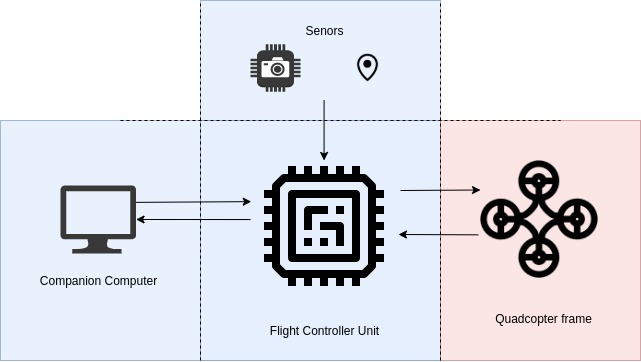
\includegraphics[scale=.55]{drone_setup}
        \caption{The typical setup for an autonomous UAV.}
        \label{fig:ds}
    \end{figure}

    Figure:~\ref{fig:ds} shows a typical setup for UAV.
    Parts of the system highlighted in blue represent systems that would be worked on during the course of this research.
    The idea is that the system being designed should provide localisation data which should be independent of the rotor build.
    These will be further scoped in the upcoming sections but it will involve doing a quality exercise of the LPS tp determine measurement uncertainty and limitations,
    writing additions or modifying the firmware of the FCU to integrate the LPS and setting up the pipelines for a companion computer to receive the pose estimates and use them.
    Additonally, the overall aim would be to get better pose estimates that would form the basis of any autonomous control and navigation.


    % Give intro to LPS, proposed setup and then plan to complete
